
\section{Algorithmic Methods for Fast Decoding} 
\label{sec:fast-decoding}

\begin{figure*}[h] 
    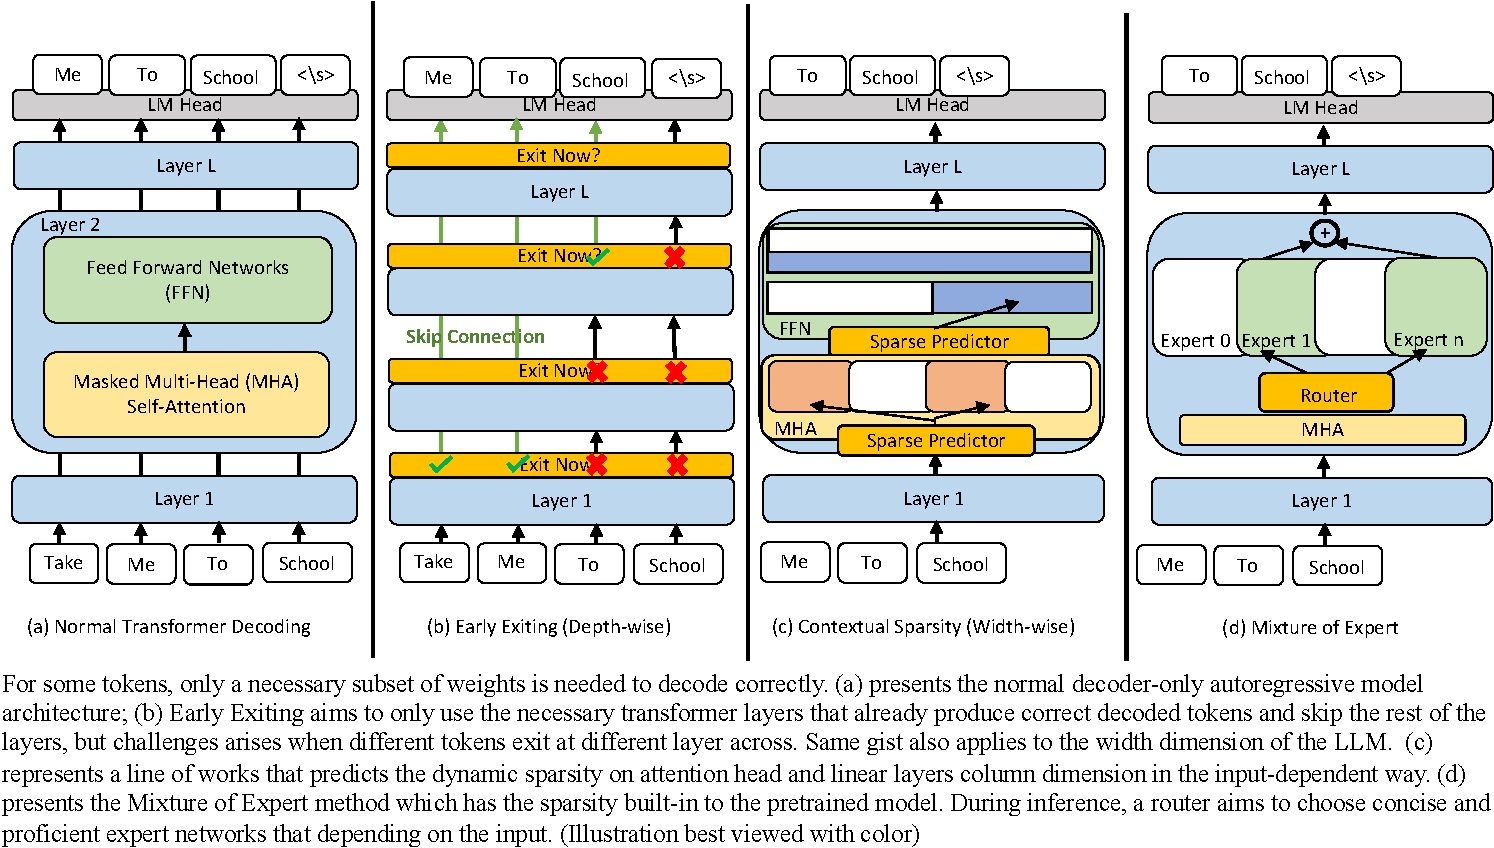
\includegraphics[width=\textwidth]{EarlyExiting.pdf} 
    \caption{Illustration of Input-Dependent Dynamic Network Technique} 
    \label{fig:early_exiting} 
\end{figure*} 

LLMs have achieved astonishing performance in various text generation tasks. They typically contain the decoder stage that generates tokens one after another, following an autoregressive relation with all preceding tokens. 
During the decoding of every token, decoder weights have to be repeatedly loaded into memory. As the parameter size of LLM becomes colossal, the decoding process becomes heavily memory-bound \citep{dejong2023fido} and experiences low hardware utilization, leading to severely long latency \citep{kim2023stack}. 
This is particularly problematic in real-world applications like ChatBot, where quick and even real-time responses are crucial. Therefore, there is a strong need to optimize the decoding process to improve performance in such applications.
% It is highly required to optimize the text generation process in real-world applications such as ChatBot \cite{openai2023gpt4} which demands swift even real-time responses. 

This section focuses on the discussion of prior efforts to reduce the LLM inference cost from an algorithm perspective. 
% We are aware of the ample previous attempts from the system and hardware perspectives and defer the discussion of them in Sections 5 and 6. 
% Also, model compression techniques introduced in Section 3 can directly reduce the parameter size of the LLM and decrease the inference latency, as LLM inference is memory-bound. 
% However, these techniques inevitably lead to performance degradation to tradeoff the model size shrinkage, which is potentially unacceptable for certain real-world applications. 
% We looks at prior works that reduce LLM inference latency but need to store the entire LLM in the machine storage to preserve the text generation quality. 
Specifically, this section intends to develop the discussion from two directions: 
\begin{itemize}
    \item In section \ref{fixedtoken}, for every single token decoded (fixed \#tokens decoded), how to utilize the minimum number of parameters of the LLM. 
    \item In section \ref{fixedparameter}, for every single forward propagation of the LLM (fixed \#parameters used) how to decode the maximum number of tokens. 

\end{itemize} 

\subsection{Minimum Parameter Used Per Token Decoded} 
\label{fixedtoken} 

Interestingly, \cite{simoulin-crabbe-2021-many} has shown that although language models tend to have a huge number of parameters, not all parameters are needed to generate the accurate tokens. LLM inference latency can be reduced by selecting only a subset of necessary parameters to use (load) per input token and still preserving the decoded token's accuracy. In this section, we look at input-dependent dynamic weights dropping scheme for LLM from three different perspectives: \ref{earlyexit} looks at early exiting, or dynamically choosing weights in the layer, depth, dimension; \ref{contextualsparsity} introduces methods that dynamically detects sparsity in the width dimension of the LLM, pruning out heads and MLP columns; \ref{mioe} present Mixture-of-Experts (MoE) which pretrains a sparse model and chooses the correct experts for the different input during runtime. 


\subsubsection{Early Exiting} \label{earlyexit} 


Early exiting (or layer skipping) has been a well-explored idea in various network architectures, particularly for the encoder-only models~\citep{baierreinio2020node, hou2020dynabert, li2021cascadebert, liu2020fastbert, liu-etal-2022-towards-efficient, schwartz-etal-2020-right, stickland2019bert, xin2020deebert, zhou2020bert, zhu-2021-leebert, schuster2021consistent}.
% However, the LLMs that specialize in continuous token generation at the sequence level rely particularly on the decoder architecture. 
Early exiting for decoder architecture requires consistency and quality retaining on the sequence level where each token depends on the previous tokens, which are considerations lacking in the previous abundant encoder-only early-exiting literature. 
The decoder contains layers of identical structure. Benefiting from this trait, the output hidden states of every layer can be used to pass in the LM Head to get a probability distribution prediction of the next token decoded. 
\cite{geva2022transformer} and \cite{simoulin-crabbe-2021-many} observe that for some tokens, the hidden states saturate during the intermediate layers. In other words, early exiting in the middle would, for some tokens, output the correct top-1 prediction as running through the full model. This observation lays the basis for the success of decoder early exiting methods. 

\cite{elbayad2020depthadaptive} conducts an early effort for efficient machine translation tasks to use early exiting on the decoder architecture. 
It proposes a general approach to follow. 
Shown in Figure~\ref{fig:early_exiting} (b), during the forward propagation, after every layer, there is an internal confidence function, usually a fixed metric or an MLP with a small number of layers, that computes a confidence score based on the hidden states on how likely it is to saturate at the current layer. The score is used to decide whether to exit through some carefully designed criteria. 
The LM Head is then used to output the next token-predicted probability distribution. 
Due to the high similarity of the newer follow-up works, we extend the discussion by looking at the key challenges of designing early exiting schemes for language models, where they introduce different novel techniques. 

\textbf{Modeling the Confidence of Saturation}. CALM \citep{schuster2022confident} studies three different ways to output the confidence score to exit: the softmax response, or the difference between the top two values after the softmax; the saturation of hidden states, or the cosine similarity between the current layer's hidden states with the last layer; the output of a linear classifier inserted to every layer. 
% To train the classifier, a small dataset (oracle) is made to collect pairs of output hidd
The linear classifier is trained by simply using a cross-entropy loss to align MLP output when inputting the hidden states with whether the top-1 token decoded as exiting on the current layer matches the top-1 token decoded of the full model. 
The experiments presented suggest that despite not being the most accurate predictor, the classifier method reaches the optimal trade-off between additional FLOPs overhead with prediction accuracy on score generating. 
Building up from CALM, \citep{bae2023fast} observed that when consistently exiting from shallow layers will result in an abnormally long length. Also, the confidence score computation on every layer injects high overhead and diminishes the benefit of early exiting. Therefore, it proposes to only have two choices for early exiting: either exit from the so-called "shallow module" or a group of shallow layers, or go all the way to the full model, or "deep module", drastically reducing the number of classifiers needed inside the model. Such design enables it to achieve more speedup than CALM, reaching 2x for certain tasks. 
On the other hand, ConsistentEE \citet{zeng2023consistentee} proposes a different method to predict when to exit. It uses an RL policy network that is iteratively trained with the per-layer output classifier head. The policy networks are trained with the goal of balancing the optimization of both efficiency (the early layer receives rewards) and accuracy (the reward function has a term that is the early exit output CE loss). 

\textbf{Early Exit Criteria}. CALM \cite{schuster2022confident} proposes a distribution-free calibration technique that uses the fixed sequence testing procedure (Family-wise Error Rate procedure) to output the suitable threshold. The threshold is exponentially decreasing to allow more aggressive exiting for tokens later in the sequence. \cite{bae2023fast}, on the other hand, observes that the pattern of confidence criteria resembles a beta distribution and uses the on-the-fly data to update a beta distribution model through MLE and use such probability model to guide its decision.
% discovers that confidence has a strong correlation with the Beta distribution and uses a Beta Distribution model to on-the-fly adapt to the dynamics. 
\cite{zeng2023consistentee} bypasses this issue by letting the policy network directly output the exit decision. 

\textbf{Hidden States Propagation}.
Hidden states of the skipped layers can pose a technical challenge. As shown in the \ref{fig:early_exiting} (b), the token position at "school" exits later than previous tokens. However, the last self-attention layer doesn't have the previous key-value pairs of the previous early exited tokens. \cite{elbayad2020depthadaptive} and \cite{schuster2022confident} proposes the "hidden states propagation" technique. For example, the hidden states of token "Max" at the exited layer $l_1$ are stored. When the later token "school" reaches deeper layer $l_2$, the hidden state for "Max" is copied for all layers between $l_1$ and $l_2$, and the key-value pairs are then computed on the copied hidden states. Basically, to approximate the deep layer's hidden state with the ones from the early layer. Later works \cite{bae2023fast} and \cite{ding2023efficiency} found that state propagation leads to performance degradation. Since LLM inferences are dominated mostly by memory loading, computation is relatively "free". These two methods proposed to recompute the later hidden states directly on the fly. \cite{chen2023eellm} proposes to run the full large model in parallel to the early exit stream to efficiently parallel the computation of the missing kv cache. \cite{din2023jump} conducts a systematic study on using a linear network to jump across layers for transformer architecture and shows that linear layers can be added to effectively bridge the performance gap between directly copying and computing the hidden states with low memory and compute cost. 
SkipDecode \cite{delcorro2023skipdecode} chooses an aggressive approach to prioritize the speedup and relax the performance preservation goal. By utilizing the observation that a token coming later in the same sequence on average requires less number of layers to decode the correct tokens, it completely bypasses the need for state propagation by forcing the maximum layer used to be monotonically decreasing for deeper positions. Besides, SkipDecode also introduces fixed exit points to optimize for batched early exit. 

\textbf{Output Classifier Training}. When exiting from intermediate layers, the intermediate hidden states need to go through an output classifier head to output prediction of the next token probability distribution. The output classifier can either be shared as shown in Figure~\ref{fig:early_exiting} or per-layer independent. These classifiers are usually trained to better adapt to the early exiting pattern. \cite{elbayad2020depthadaptive} proposed to have an average CE loss of all layers to be the training loss of the classifier. On the other hand, \cite{schuster2022confident} uses a weighted average where weights increase as the layer number increases, assigning more contribution to deeper layers. \cite{bae2023fast} introduces a dynamic knowledge distillation loss which dynamically assigns the "shallow module" a suitable hidden state from the "deep module". Both \cite{rotem2023finding} and \cite{ji-etal-2023-early} find a "conflicting gradient" issue when joint training with the same loss across all models: \cite{rotem2023finding} detects the gradient conflict between early and later layers of language models, while \cite{ji-etal-2023-early} spots the "orthogonal gradient" between the objective to improve semantic awareness and the objective to improve early exciting decision. Both methods propose adding an additional block of parameters and iterative training to alleviate the issue. 
Besides the above-mentioned perspectives, \cite{chen2023eellm} studies system-level optimization techniques to efficiently run LLM early exit under the 3D parallelism setting. 

% On the other hand, ConsistentEE \cite{zeng2023consistentee} proposes a different method to train the internal classifier. It observes that for the shallower layers, internal classifiers usually perform badly, potentially contributing to a globally undesirable decision. To improve the training, this method first relaxes the constraint that only one classifier across all the layers is required to predict the existing decision correctly. 
% \cite{delcorro2023skipdecode} takes an aggressive approach to prioritize the speedup and relax the performance preservation goal. To enable better fficiency on the batch dimension, 

\begin{figure*}[ht] 
    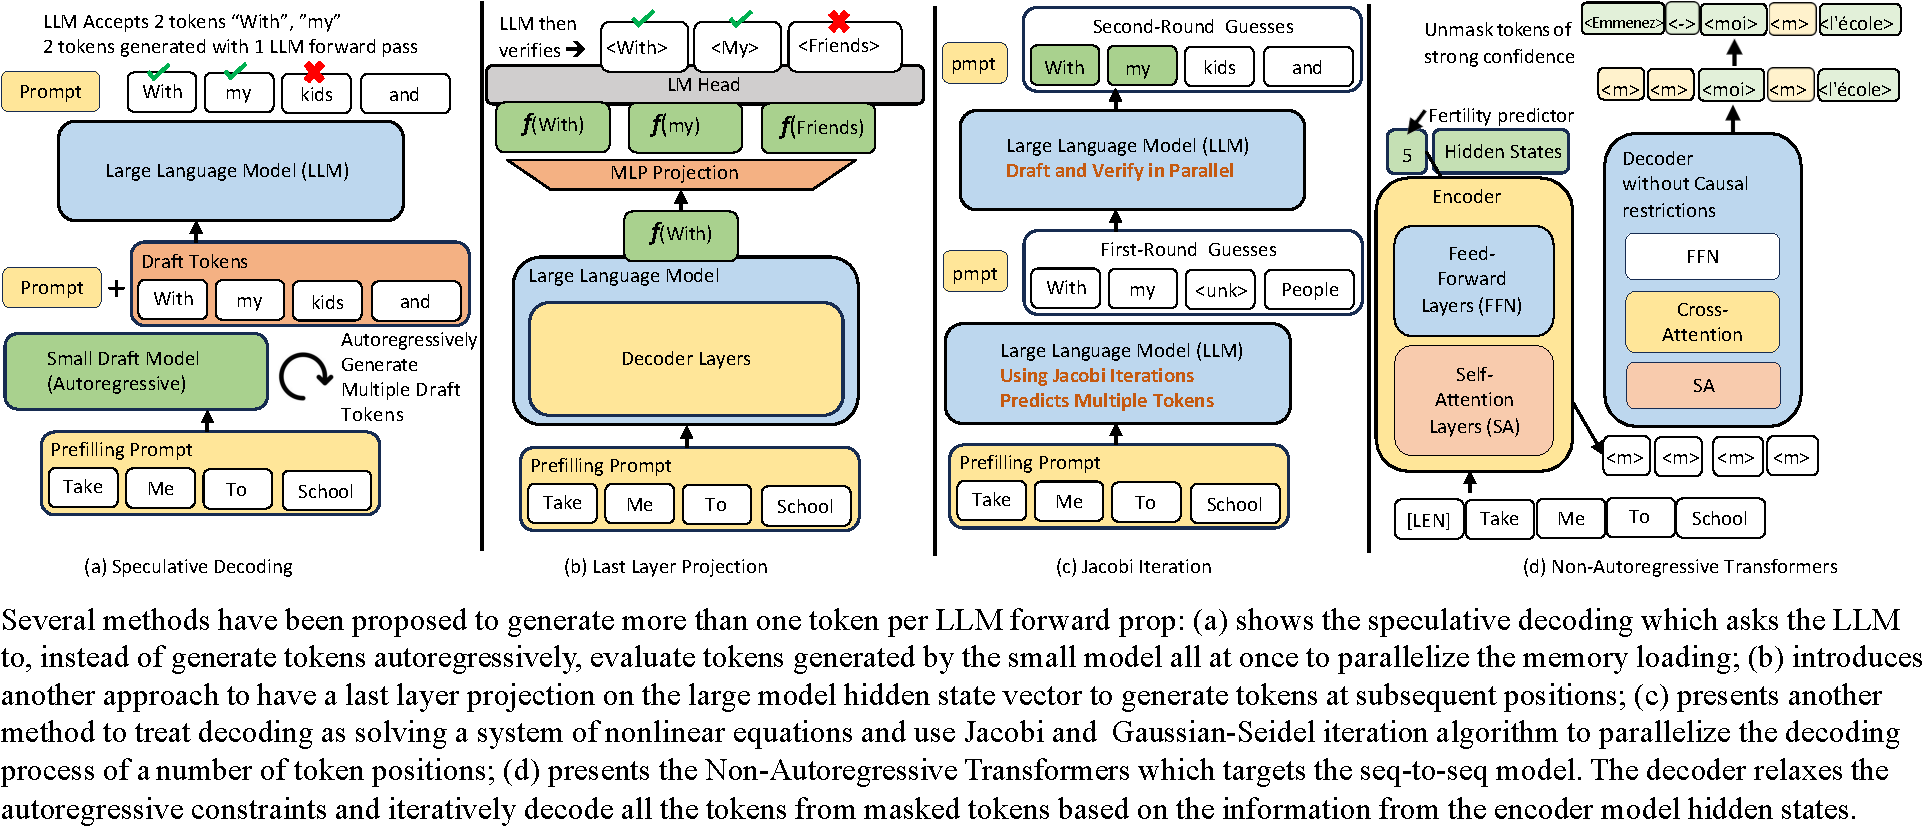
\includegraphics[width=\textwidth]{specudec.pdf} 
    \caption{Illustration of the Parallel Decoding Methods} 
    \label{fig:specudec} 
\end{figure*} 


\subsubsection{Contextual Sparsity} \label{contextualsparsity} 

While early exiting aims to select parameters on the depth dimension, some techniques have also been proposed to exploit the dynamic sparsity on the width dimension. Deja Vu \cite{liu2023deja} conducts a comprehensive study on dynamic sparsity on the LLM width dimension. The paper reveals that contextual sparsity can go up as high as 80\%, meaning that the majority of the weights can be left out while still preserving the original model performance. However, the chosen weights are dynamic and different for different input tokens. The paper formulates this problem as a nearly neighbor search problem that for a given hidden state from the embedding layer of previous layers, how to find the attention heads and the MLP columns that are the most similar to these tokens. To save compute, the paper proposes to train a small MLP network as the Sparse Predictor in front of the Multi-Head Attention (MHA) and the Feed-Forward Networks (FFN) of the LLM, shown in Figure~\ref{fig:early_exiting} (c). By using only a subset of weights and reducing the memory IO overhead, Deja Vu manages to achieve over 2x speedup of LLM inference. Building on Deja Vu, PowerInfer (\cite{song2023powerinfer}) brings the contextual sparsity finding to the LLM inference across heterogeneous devices (CPUs and GPUs). PowerInfer discovers a substantial portion of weights are heavily used and activated in the input-independent setting, thus stored on the GPU memory, while others are on the CPU memory. 
% The paper first identifies part of the neurons (columns and rows) are heavily activated and used (input-independent), while some are activated for some input. The first chunk are loaded on GPU memory, while the second chunk will always be stored on the CPU memory. 
Then, to specifically find the weights to use for a given input token, it trains a smaller sparse prediction than Deja Vu. To make the sparse predictor, it initializes the sparse predictor to have a dynamic structure and iteratively trains and modifies the sparse predictor. 
% Then, it trains a Deja Vu-like sparse predictor for identifying which part of the model should be computed. 
To better do inference of the model deployed on the mixed CPU and GPU environment, it introduces a novel memory placement scheme and implements a vector-based sparse computation library. 
% To eliminate the size of such predictor, it uses an adaptive training schedule to train variable sized predictor for different layers. Then, to better perform mixed CPU-GPU model, it introduces novel memory placement method and separate sparse computation schemes for both. 
Concurrently, MatFormer (\cite{devvrit2023matformer}) studies the problem of LLM deployment on various heterogenous devices of different hardware capabilities. They added dynamic structure only on the FFN, which occupies 60\% of total weights. The model is specially trained so that during inference, based on the target hardware properties, MLP layers are sampled on the row dimension to give a model of various sizes with reasonable performance. 
% MLP layers there sliced on the row dimension evenly, and a subset of weights is sampled based on the hardware properties for inference without retraining. 
To diversify the model size selection, it imposes a Mix’n’Match method to choose different settings for different layers, so combined would give a more variable model size. 
% The technique has been tested on both ViT and LLM with either decoder-only or encoder-decoder models. 


\subsubsection{Mixture-of-Expert Models} \label{mioe} 
Language Models, especially transformer architecture, exhibit strong power-law scaling (\cite{kaplan2020scaling}, \cite{hoffmann2022training}) of performance when the training dataset is scaled up. On the other hand, though bringing strong performance gain, the large parameter count makes training and inference of the model inefficient. The mixture of expert (MoE) technique is a well-studied topic (\cite{6215056}) that effectively decouples the parameter count of the model and the computation FLOPs required by the model training and inference, thus bringing huge gains of efficiency under certain conditions. Further, MoE is shown to effectively scale up the language model size and increase its performance without the concern of increasing compute during inference (\cite{lepikhin2020gshard}, \cite{fedus2021switch}). Shown in Figure \ref{fig:early_exiting} (d), an expert network is inserted into the transformer architecture to replace the FFN layers. Also, a gating function is introduced between the Multi-Head Attention and the expert network which aims to select the best-fit expert or experts for the given input token. For in-depth analysis and discussion about the MoE scaling generalization, routing algorithms, training techniques, etc., we refer the readers to the survey on Sparse Expert Models (\cite{fedus2022review}). 
\textit{Although both rely on the input token to determine sparse structure, We deliberately separate MoE and the contextual sparsity techniques because the latter operates on pre-trained dense language models and exploits the sparsity from the dense neural networks, while the prior trains a sparse model from the beginning.} 
More recently, MoE techniques have achieved substantial success. Sparse Mixer (\cite{lee2022sparse}) brings 89\% and 98\% speedup in both training and inference to BERT (\cite{devlin2019bert}) models. \cite{du2022glam} uses only 49\% FLOPs but beats GPT-3 (\cite{brown2020language}) in performance. ST-MoE (\cite{zoph2022st}) brings MoE to the encoder-decoder models, even becoming the state-of-the-art model for many reasoning and generation tasks. ST-MoE, using 
20x and 40x fewer FLOPs in training and inference, beats 540B PaLM (\cite{chowdhery2022palm}) in performance. Mixtral 8x7B (\cite{jiang2024mixtral}), while only actively using 13B parameters during inference, performs on par with Llama2-70B models (\cite{touvron2023llama2}) across various evaluation benchmarks. 

Besides, various attempts have been made to optimize MoE model inference. \cite{kossmann2022optimizing} builds an efficient compiler library RECOMPILE for MoE models that introduce dynamic recompiling and optimization according to varying inference batch sizes. \cite{rajbhandari2022deepspeed} extends the ZeRO distributed inference method to MoE models. \cite{jawahar2023automoe} conducts Neural Architecture Search (NAS) on the expert network architecture. \cite{yi2023edgemoe} deploys large MoE language models on the edge devices. It optimizes the deployment around the finding that some neurons are much more heavily used in the MoE models than others. 

\subsubsection{Roofline Model Analysis for Dynamic Parameter Reducing}

% Minimum Parameter Used Per Token Decoded 的方法在每次推理的时候，相当于把一个较大的网络变成一个较小的网络。可以同时降低计算和memory access开销，因此每个算子的Arithemetic Intensity变化不大，bound的类型也变化不大。对于Early Exiting或者Layer Skipping来说，由于整个Transformer Layer被跳过，所以整体的计算量、访存量、推理时间的降低是几乎等比例的。也就是说，当网络中跳过了多少层，网络的推理时间就会减少多少。对于Contextual Sparsity和Mixture of Expert这样的方法来说，由于不同MHA和FFN中的不同层的arithmetic intensity不同，跳过他们带来的计算量和访存量的变化也不同，因此最终推理时间的变化也会不同。

The Minimum Parameter Used Per Token Decoded methods simultaneously decrease computational and memory access overhead. From the viewpoint of roofline model, these methods result in small changes to the arithmetic intensity of each operator and the type of bound.

For Early Exiting or Layer Skipping methods, entire Transformer layers are skipped, leading to a proportional reduction in overall computation, memory access, and inference time. In other words, the inference time decreases proportionally to the number of layers skipped in the network.
However, for methods like Contextual Sparsity and Mixture of Experts, the arithmetic intensity varies across different operations. Consequently, dynamically choose to activate these layers leads to varying reductions in computation and memory access, resulting in different impacts on the overall inference time.
% As shown in Figure~\ref{}, we demonstrated


\subsection{Maximum Tokens Decoded Per LLM Forward Propagation} 
\label{fixedparameter}

Another angle to reduce the latency of LLM inference is to relax the LLM from the limitation of autoregressive decoding and have more than one token decoded per one LLM forward propagation. We look at two ways to achieve it: \ref{specdec} presents the speculative decoding method which introduces a computationally efficient draft model to propose candidates for the next few token positions, while the LLM is used to evaluate the draft model's proposed draft tokens, instead of generating next tokens. 
On the other hand, \ref{pd} presents works that enable the LLM to directly decode multiple tokens from a single forward propagation. Due to some methods combining the benefits from both directions and lying in the middle, we manually add a distinction just for the sense of nomenclature that speculative decoding methods here all have the draft model to be in the transformer architecture. 

\subsubsection{Speculative Decoding} \label{specdec} 

Due to the demanding memory loading challenges and autoregressive properties, LLMs are inefficient in inference. However, models that are much smaller in size are shown (\cite{kim2023speculative}) to have the ability to decode the correct sequences as the LLM, as long as some key tokens in the sequence of the small model generation are corrected. Then, shown in Figure \ref{fig:specudec} (a), when the small model is asked to infer (speculate) and output a sequence of draft tokens, memory loading of model weights is less of a problem, resulting in much higher utilization in hardware computation units. To ensure the quality of the text generated by the small model, the LLM can "periodically" evaluate and correct tokens from the small model's draft. Then, although the large model needs to sometimes evaluate the wrong draft tokens, potentially leading to larger FLOPs spent than LLM autoregressive decoding, the memory loading of weights is parallelized on the token dimension and drastically reduces the memory IO overhead. Since the LLM inference is memory bottlenecked, the speculative decoding will potentially reduce the LLM inference latency greatly. 

\textbf{LLM Distribution Preserving} During early exploration of this idea, two different paths emerged concurrently. \cite{kim2023speculative} proposed to have the small model speculate and generate draft tokens until the token decoded confidence falls below a threshold. Then, the small model "fallback" to the large model to evaluate the draft tokens generated and hand over to the small model. Some of the tokens are rejected, so the large model asks the small model to "roll back" these wrong tokens and resume speculating. In the paper's setting, all decoding is "greedy". The paper show that the large and small model pair can generate text with quality on par with the original large model autoregressive generated text. However, \cite{leviathan2023fast} and \cite{chen2023accelerating}, upon the small model speculate paradigm, points out a technique of resampling that at the position where the LLM rejects the small model's prediction that provably enables the large and the small model predictions to be in the same probability distribution as the large model's autoregressive generation. 
% TODO: elaborate on this part more 
The following techniques generally follow the paradigm of speculating then evaluating and resampling to preserve the LLM autoregressive decoding quality while enabling speedup. 
% are in much higher utilizatio 

\textbf{Building a Tree of Draft Tokens} Since the LLM generates in the autoregressive order, every token is dependent on all previous tokens generated, and the length of the accepted tokens in the small model's draft is usually modest and bounded. It is exponentially more difficult to speculate on tokens more distant in the future. For example, if the small model is asked to output the length m draft sequence, and the LLM accepts n, n $<$ m, the (m - n) tokens are automatically discarded. 
Thus, the speedup ratio of speculative decoding is modest, since every LLM forward leads to only a limited number of tokens being decoded. 
% Thus, the higher acceptance rate leads to a better speedup ratio achieved. 
There are two ways to improve the speedup of speculative decoding. First, \cite{sun2023spectr}, \cite{miao2023specinfer}, and \cite{xu2023llmcad} all proposed to boost the draft on the batch size direction, or letting the small model sample multiple plausible draft sequences for the LLM to evaluate in parallel. Specifically, \cite{sun2023spectr} proposes a way and theoretical guarantees for the LLMs to batch verify and resample from the multiple small model drafts so that the LLM distribution is preserved and no loss of generation quality is incurred. The paper first connects speculative decoding to the broader problem of discrete optimal transport. The small model is asked to sample multiple draft sequences using topk sampling. Based on the properties of the discrete optimal transport, finding the optimal method to evaluate and resample becomes finding the optimal transport path. On the other hand, besides from maintaining the speculative decoding consistency of draft trees, \cite{miao2023specinfer} constructs the token tree not based on the top predictions from the small draft model, but based on multiple diversely trained small draft models, each running in parallel and output diverse but powerful draft sequences. The paper proposes a novel draft token tree construction algorithm that builds a tree of candidate tokens based on the diverse draft sequences through predefined expanding and merging schemes. Then, the large model is asked to parallel verify the constructed tree using a carefully designed tree attention to maximize the reuse of the key-value cache and maintain a tree-based causal mask. \cite{xu2023llmcad} innovatively applies the benefit of speculative decoding to edge devices. The paper builds an LLM serving engine for the edge, where a smaller draft LLM is sitting consistently in memory, while a larger robust LLM is occasionally loaded in memory to do verification. To boost the acceptance rate from the large LLM, it also constructs a tree using topk tokens. To cater to the edge hardware characteristics, it implements a tree-based parallel verification decoder equipped with masking and a customized large-small LLM computation pipeline to avoid memory contention. 

\textbf{Knowledge Distillation and Self-Speculative Decoding} Another way to improve the acceptance rate is to improve the small draft model's ability to align with the LLM's generation distribution, which can be done through finetuning the small models on corpus generated by the large models with knowledge distillation. 
% \cite{zhou2023distillspec} and \cite{liu2023online} directly finetune the small model through knowledge distillation from the target LLMs. 
\cite{zhou2023distillspec} establishes a mathematical connection between the acceptance rate and natural divergence between the small model and the LLM: minimizing the divergence is maximizing the acceptance rate. The paper also studies a range of different knowledge distillation losses and shows that adding knowledge distillation brings consistent 10-45\% improvement in latency speedup. However, the paper generally finds that the optimal knowledge distillation loss choices vary model by model and should be tuned as a hyperparameter. \cite{liu2023online} also shows that knowledge distillation boosts the small model training. Besides, the paper brings speculative decoding to the cloud online learning settings. LLM inference is memory-bottlenecked, which means that there is always a surplus in computation resources. 
The compute can be used to train a draft model continously on server, which brings two benefits: Continuously training with knowledge distillation boosts its acceptance rate and, thus, reduces the LLM inference latency; 2) serving input is constantly shifting in domains, and continuous training helps the draft models maintain the strong performance in different domains. 
% The paper also shows knowledge distillation can be successfully added to boost the small model and further build a prototype of the said online speculative decoding. 
\cite{zhang2023draft} avoids storing a separate draft model by selectively sampling a smaller draft model from the large model itself. Before deployment, the paper utilizes a Bayesian optimization method to search for a draft model by skipping intermediate layers within the pretrained large model. Besides, it proposes an adaptive threshold selection technique tailored for the decoding of the draft model sampled from the large models. 

\subsubsection{Parallel Decoding} \label{pd} 

Alternatively, abundant works have been proposed to enable the large model to directly perform parallel decoding without the help of a small transformer model. 

\textbf{Simultaneously Predicting Multiple Future Tokens} A wide variety of works are exploring the subject of enabling multiple token predictions directly from one forward pass of the Large Language Model. \cite{stern2018blockwise} pioneers the design of inserting a linear projecting layer between the last hidden states output and the input of the language modeling head to enable multiple future tokens to be projected solely based on the current token's last hidden states as input. Evaluation is subsequently made by the LLM to decide whether to accept or reject these projected tokens. The proposed technique focuses on the sequence-to-sequence models that have the decoder structure. 
More recently, \cite{cai2024medusa} extends the previous work to the decoder-only language models as shown in Figure \ref{fig:specudec} (b). Besides the last layer projection, to further improve the decoded acceptance rate, the paper proposes to add a tree-based decoding structure and the associate attention mask design to propose multiple drafts simultaneously for the large model to evaluate. 
Besides, concurrently \cite{monea2023pass} proposes to add several dummy tokens at the end of the input sequence are called "lookahead embeddings" in work. 
During the forward pass of each layer, the information of previous prompt tokens and already decoded tokens can be used to parallel decode several consecutive future tokens. 
To enable this design, the work trains a separate embedding layer that specifically serves these lookahead embeddings. \cite{li2024eagle} also aims to do parallel decoding with LLM evaluation. Like previous works, it also adds a lightweight structure FeatExtrapolator. Differently, the structure takes both the previous token's last layer hidden states and the actual decoded token embedding as input and output the hidden states prediction of the next layer. The LM head of the LLM is used, and several tokens are sampled, which are then used to build a decoding tree for the LLM to evaluate in parallel. 

\textbf{Retrieval of Frequent N-grams} Besides directly using the LLM to output several following tokens, some works use the frequently appeared n-grams in natural language to enable multiple future tokens to be generated within one forward pass of the large model. LLMA (\cite{yang2023inference}) first observes that the generation tasks tend to ask the LLM to repeat tokens that appeared in the previous contexts. Based on this information, the paper set out to use the decoded tokens and the prompt to do prefix matching with a set of reference documents so that if a repetition occurs, tokens that are repeated can be directly copied to the current place. Then, an LLM will evaluate these found candidate tokens from the previous context to decide whether to use them. \cite{he2023rest} further extends LLMA and proposes to first construct a database of common phrases based on the LLM pretrained or finetuned dataset and corpus. Then, during decoding, the previous context prompts or tokens are used as the query to be used to retrieve into the constructed database. The candidates retrieved are organized into a prefix tree structure or a trie, which the LLM can then evaluate efficiently. \cite{lan2023copy} similarly follows to use the retrieval methods to speed up inference. In contrast, it adds an extra attention layer at the end of the LLM to use the current context represented by the hidden states of the current token as the query to attend to relevant phrases retrieved from the documents of reference and select top phrases based on the attention scores. 

\textbf{Hierarchical Structure In Language} Hierarchical Structure exists in language. For writing a long piece of article, the usual approach is to first write out the general outline of the paper, as in the format of bulletin points. Then, for every bulletin point, arguments can be extended to encapsulate the full intent of the bulletin point. Based on the observation that arguments for different bulletin points are relatively independent in semantics, some methods are proposed to parallelize the generation process for different bulletin points. Skeleton-of-Thoughts (\cite{ning2023skeletonofthought}) proposed to first ask the LLM to generate concise bulletin points for an article, and then collect these bulletin points on the batch axis and feed them into the LLM again as a prompt to ask the LLM to expand the arguments for each bulletin points in parallel. The achieved speedup is approximately 2x, but with the caveat that the method cannot easily generalize to all text generation tasks. More recently, APAR (\cite{liu2024apar}) extends upon this direction. The paper adds specific soft tokens that explicitly inform the LLM of the hierarchical information during the generation. The LLM is further instruct-tuned to incorporate the added special tokens, and the generation is boosted with the Medusa (\cite{cai2024medusa}) technique to achieve 4x speedup on text generation with the hierarchical structure. 

\textbf{Jacobi and Gaussian-Seidel Iterative Algorithms} \cite{pmlr-v139-song21a} pioneers the study of using parallelizable methods to approximate the results from iterative and sequential inferences of fully connected networks or CNNs. Though seemingly in-viable, the paper finds that neural networks can tolerate numerical approximation errors and the data patterns that neural networks learn expose parallel structures to some extent, which makes it possible in some scenarios to parallelize the sequential inference of neural networks. 
Jacobi and Gaussian-Seidel Algorithms were previously proposed to solve a system of non-linear equations (\cite{ortega2000iterative}) and are shown to effectively parallelize the sequential neural network inference. \cite{santilli2023accelerating} extends the Jacobi and Gaussian-Seidel algorithms to parallelize the autoregressive decoding in the Machine Translation tasks. Specifically, this work is built on top of the previous Non-Autoregressive Transformers architecture (which we will cover later in the chapter) to enhance the parallel decoding with GS-Jacobi algorithms. The parallel decoding process stops when a [EOS] token is found in the decoded text. Concurrently, Lookahead decoding (\cite{fu2023lookahead}) shown in Figure \ref{fig:specudec} (c) extends this method to parallelize the LLM generation of subsequent tokens. Besides using the vanilla Jacobi iterative algorithm, it also boosts its speed with a retrieval-based algorithm to reuse the previously seen n-grams. In addition, it parallelizes the lookahead step and LLM verification step by introducing a carefully designed attention mask to the original LLM model to further improve decoding efficiency. 

\textbf{Non-Autoregressive Transformers} For Machine Translation tasks that require autoregressive decoding of the sequence-to-sequence model, Non-Autoregressive Transformers (NAT) has been proposed to iteratively decode all of the output tokens together, as shown in Figure \ref{fig:specudec} (d). NAT has been relatively well-explored (\cite{gu2017non}, \cite{wang2019non}, \cite{li2019hint}, \cite{sun2019fast}, \cite{wei2019imitation}, \cite{shao2020minimizing}, \cite{lee2018deterministic}, \cite{ghazvininejad2019maskpredict}, \cite{guo-etal-2020-jointly}, \cite{gu2020fully}, \cite{savinov2021step}), and we point the readers to the following survey paper that covers specifically NAT models \cite{xiao2023survey} for an in-depth review and analysis on the subject. 
Coarsely, the speedup of text decoding comes from making a single forward pass of the decoder output more than one token. The input sequence is first fed into the encoder, which outputs the hidden states that extract the input semantics. The output hidden states of the encoder are then used as the condition for the decoder pass. To speed up the text generation, the decoder side relaxes the autoregressive constraints and takes a sequence full of dummy tokens [pad] as the input to start the iterative parallel decoding process. During each iteration, based on the condition set by the encoder output hidden states, some tokens can be confidently predicted, which are unmasked. 
The sequence is mixed with unmasked decoded tokens and the remaining masked tokens are fed to the decoder again until every token is decoded. 
The length of the sequence fed into the decoder, or fertility, is usually learned either inside the encoder as a special [CLS] token or by a specialized fertility predictor between the encoder and the decoder. More recently, \cite{savinov2021step} treats the decoder as a diffusion model and trains it to denoise the noisy initial sequence based on the conditions given. However, because of the requirement to use encoder hidden states as the condition for parallel decoding, NAT methods face natural difficulties in extending directly to decoder-only architectures. 

% many works observed that finding draft tokens is difficult since within the memory budget allowed for the small model, it is hard to construct the small model produces 
